% !TeX program = xelatex
\documentclass[12pt,a4paper]{article}
\usepackage{fontspec}
\setmainfont{Times New Roman}
\usepackage[english,russian]{babel}
\usepackage{amsmath,amssymb,mathrsfs,cancel}
\usepackage[margin=22mm]{geometry}
\usepackage{graphicx,float}
\usepackage[unicode,hidelinks]{hyperref}
\DeclareMathOperator{\grad}{grad}
\DeclareMathOperator{\Div}{div}
\newcommand{\Rey}{\mathrm{Re}}
\setlength{\emergencystretch}{3em}
\sloppy
\interfootnotelinepenalty=10000
\newcommand{\topic}[1]{\par\medskip\noindent\textbf{#1}\par\nobreak\smallskip}
\renewcommand{\thefootnote}{\arabic{footnote})}
\begin{document}
\section*{Вопрос 12}
Понятие об эволюционности разрывов для гиперболических уравнений. Эволюционность скачка насыщенности в задаче Бакли — Леверетта. Модель двухфазных течений с учетом капиллярной разности давлений. Понятие об уравнении Рапопорта — Лиса. Представление о задаче о структуре скачка насыщенности.

\medskip
\noindent\textbf{Источник:} А. Г. Куликовский, Е. И. Свешникова. \textit{Нелинейные волны в упругих телах}. Москва: Московский лицей, 1998. § 1.3, с. 26--31; К. С. Басниев, А. М. Власов, И. Н. Кочина, В. М. Максимов. \textit{Подземная гидравлика}. Москва: Недра, 1986. гл. 9, фрагменты с. 207, 210, 219--220; Г. И. Баренблатт, В. М. Ентов, В. М. Рыжик. \textit{Теория нестационарной фильтрации жидкости и газа}. Москва: Недра, 1972. гл. VI, § 2 (определения), § 3 (начало), с. 157, 159, 164--167; рисунок VI.11 на с. 168.
\par\bigskip
\section*{А. Г. Куликовский, Е. И. Свешникова. Нелинейные волны в упругих телах}
\subsection*{1.3. Граничные условия. Эволюционность}
% Источник: Kulikovskii-Sveshnikova.djvu; печатная страница: 26; страница файла: 26
Во многих случаях требуется найти решение системы уравнений в ограниченной области изменения $x$ или в примыкающих одна к другой областях с одинаковыми или разными системами уравнений, действующими в этих областях. Тогда для построения однозначного решения нужно задавать, кроме \textit{начальных} условий, еще \textit{граничные условия} --- некоторые соотношения, связывающие функции $u_j$ на границе.

Рассмотрим сначала вопрос о \textit{необходимом числе граничных условий для однозначного построения решений линейных гиперболических систем} уравнений с постоянными коэффициентами при наличии начальных условий.

Пусть имеется граница, положение которой задано ее законом движения $x=X(t)$ или скоростью $dX/dt=W(t)$. Функции $u_i$ считаются заданными в момент времени $t_0$ при $x>X(t_0)$ (начальные условия). Требуется построить решение системы (1.6) при $t>t_0$ в области $x\ge X(t)$. В этом случае может оказаться,
% Источник: Kulikovskii-Sveshnikova.djvu; печатная страница: 27; страница файла: 27
что некоторые из волн, содержащихся в решении (1.12), приносят в точку $x,t$ значения своих амплитуд $w_m$ не из области начальных данных, а с указанной границы, и чтобы найти однозначное решение в этой точке, надо знать значения амплитуд этих волн на границе (\textit{начально-краевая задача}).

Закон движения границы $x=X(t)$ на плоскости $x,t$ представлен жирной линией на рис. \ref{q12:fig-1-2}, наклон которой определен скоростью $W$. Будем сначала предполагать, что скорость границы $W$ не совпадает ни с одной из характеристических скоростей системы (1.6), т.е. $W\ne c^{(m)}$, $m=1,\ldots,n$. Тогда все $n$ характеристик (и соответствующие им бегущие волны) в каждой точке границы можно разделить на \textit{характеристики, уходящие от границы} в область $x>X(t)$, для которых $c^{(r)}>W$, $r=1,2,\ldots,s$, и \textit{характеристики, приходящие к границе}, для которых $c^{(l)}<W$, $l=s+1,\ldots,n$. На рис. \ref{q12:fig-1-2} характеристики изображены прямыми со стрелками в направлении роста $t$. На приходящих характеристиках известны из начальных условий значения инвариантов Римана $w_l$. Для построения решения (1.12) нужно знать значения остальных функций $w_r$ ($r=1,\ldots,s$) на уходящих от границы характеристиках.

Таким образом, для однозначного продолжения решения в области $t>t_0$ нужно так задать граничные условия, чтобы на кривой $x=X(t)$ они позволили найти $s$ значений инвариантов Римана уходящих волн $w_r$ по известным значениям инвариантов Римана приходящих волн $w_l$, т.е. $w_r=\varphi_r(w_{s+1},\ldots,w_n)$, $r=1,2,\ldots,s$. Для этого число соотношений, задающих связи между функциями $w_j$ плюс закон движения границы должно быть равно $s+1$.

Часто в задачах механики движение границы не задано, но имеется выражение для ее скорости $W$ через функции $u_i$, а связи между неизвестными функциями на границе включают и величину $W$. В этом случае все $s+1$ соотношения становятся равноправными. В исходных переменных $u_i$ они могут быть записаны в виде
\begin{equation}\Phi_q(u_1,\ldots,u_k,W)=0.\tag{1.16}\label{q12:eq-1-16}\end{equation}
% Источник: Kulikovskii-Sveshnikova.djvu; печатная страница: 28; страница файла: 28
\renewcommand{\thefigure}{1.\arabic{figure}}\setcounter{figure}{1}
\begin{figure}[H]\centering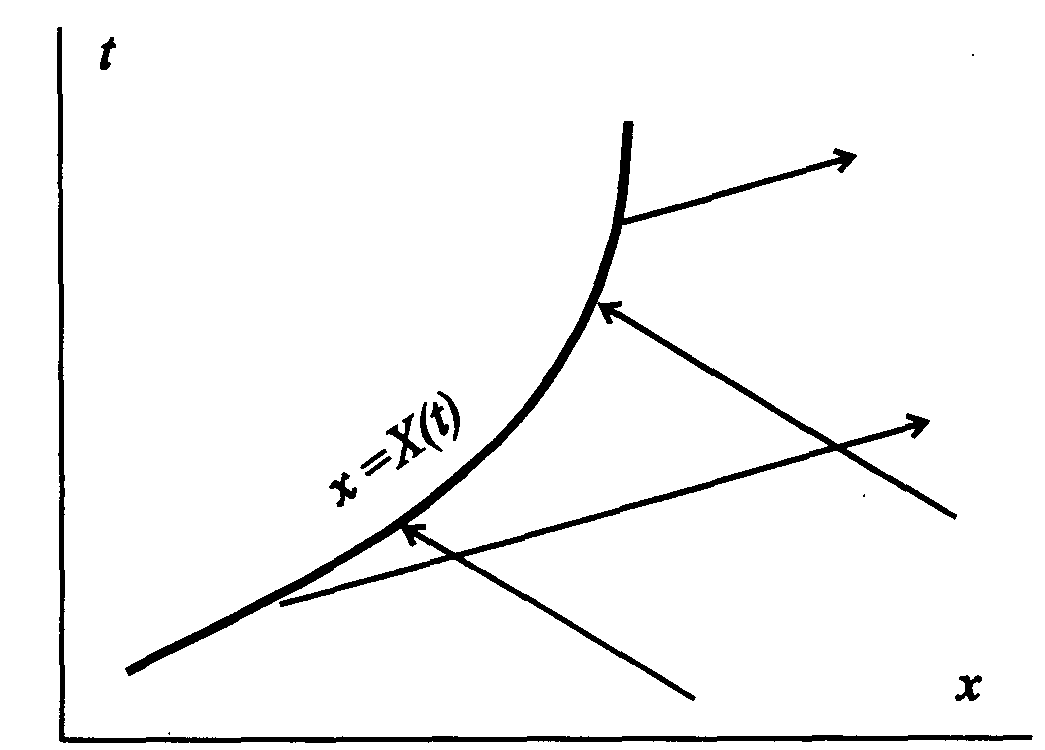
\includegraphics[width=.65\linewidth]{figures/fig-1-2.png}\caption{}\label{q12:fig-1-2}\end{figure}
Эти соотношения должны позволить найти $s+1$ неизвестную величину $w_1,w_2,\ldots,w_s,W$. Кроме того, следствием этих уравнений не должно быть никакое соотношение, связывающее между собой амплитуды приходящих волн $w_{s+1},\ldots,w_n$, так как эта связь будет противоречить произвольности начальных условий, определяющих эти величины. Чтобы это было возможно, необходимо, чтобы система \eqref{q12:eq-1-16} содержала $s+1$ уравнение с отличным от нуля якобианом относительно $w_r$ и $W$, $r=1,2,\ldots,s$.

Таким образом, \textit{для однозначной разрешимости начально-краевой задачи для линейной гиперболической системы необходимо задавать $s+1$ граничных условий вида} \eqref{q12:eq-1-16}, обладающих отличным от нуля якобианом относительно $w_1,w_2,\ldots,w_s$ и $W$, где $s$ --- число характеристик, уходящих от границы в рассматриваемой точке $x,t$. Такие \textit{граничные условия называются эволюционными}. Часто говорят об эволюционной границе, имея в виду то же самое.

Бывают задачи с таким законом движения границы, что необходимое для эволюционности количество условий может
% Источник: Kulikovskii-Sveshnikova.djvu; печатная страница: 29; страница файла: 29
меняться вдоль линии $x=X(t)$. Это происходит тогда, когда на ней есть точки, где какая-либо из величин $W-c^{(m)}$ меняет знак. Иллюстрация такого положения для системы двух уравнений ($n=2$) приведена на рис. \ref{q12:fig-1-3}. На участке границы $AB$ оба семейства характеристик приходящие, и требуемое условиями эволюционности одно граничное условие служит для определения закона движения. На участке $BD$ надо задать еще одно условие, на участке $DF$ --- два.
\begin{figure}[H]\centering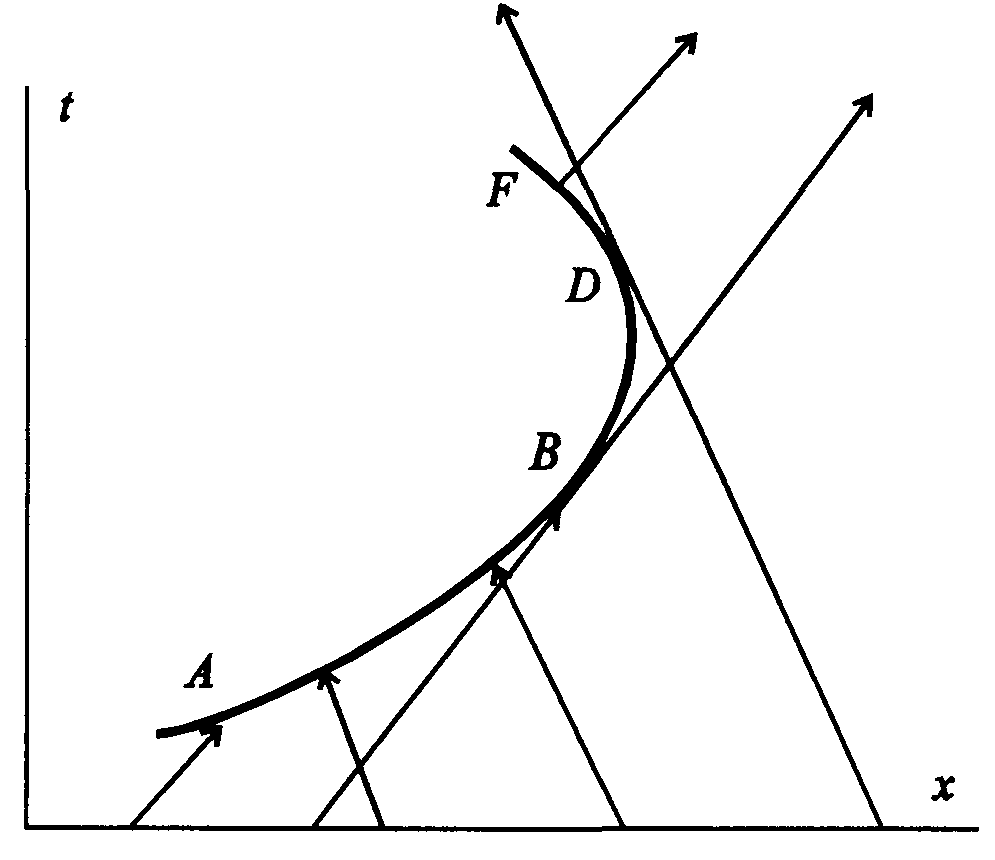
\includegraphics[width=.65\linewidth]{figures/fig-1-3.png}\caption{}\label{q12:fig-1-3}\end{figure}
В некоторых случаях граничные условия должны выставляться на границе, разделяющей области, в каждой из которых решение описывается своей гиперболической системой (это могут быть, в частности, системы и с различным числом неизвестных). В этом случае условие эволюционности границы остается прежним, однако под $s$ следует понимать число всех уходящих в обе стороны от границы характеристик (налево уходят характеристики, у которых скорость меньше, чем $W$).

Отметим здесь особый случай, играющий, однако, в силу некоторых причин, связанных с симметрией ряда важных задач,
% Источник: Kulikovskii-Sveshnikova.djvu; печатная страница: 30; страница файла: 30
заметную роль в теории. Предположим, что система соотношений, предназначенная для определения величин $w_1,w_2,\ldots,w_s,W$ на границе, распадается на независимые подсистемы. Тогда условие эволюционности граничных условий заключается в равенстве числа соотношений в каждой из подсистем числу определяемых из этой подсистемы неизвестных (при отличии от нуля соответствующих якобианов). Этот вопрос будет подробно рассматриваться в связи с условиями на разрывах решений (§ 1.6).

\textit{Для нелинейных задач под условиями эволюционности границы подразумевается выполнение условий эволюционности для линеаризованной задачи}. Линеаризация производится в малой окрестности точки на границе, в которой $u_i=u_i^0=\mathrm{const}$, так что $u_i=u_i^0+v_i(x,t)$, при этом $v_i$ малы.

Эволюционность означает существование однозначного решения задачи о взаимодействии границы с малыми возмущениями в рамках линеаризованной постановки задачи для функций $v_i$ и $\delta W$, где $\delta W$ --- малое возмущение скорости границы.

Нарушение условий эволюционности означает, что линеаризованная (или линейная) задача о взаимодействии малых возмущений с границей или имеет неоднозначное решение или неразрешима. Если число независимых граничных условий недостаточно для однозначного определения уходящих возмущений и возмущения скорости границы $W$, то решение задачи содержит произвол. Обычно это связано с физической нереальностью таких граничных условий (решения правильно поставленных задач не должны содержать произвольных функций). Более глубокое рассмотрение физической сущности проблемы иногда приводит к постановке заранее не очевидных дополнительных граничных условий (см. § 1.14, § 1.15), которые делают рассматриваемую границу эволюционной.

Линейная задача неразрешима, когда число имеющихся граничных условий превышает $s+1$. В нелинейной постановке решение правильно поставленной задачи должно существовать. Это означает, что взаимодействие границы с малыми возмущениями приводит к немалым по величине возмущениям, например, к распаду неэволюционного разрыва (см. § 1.8, а также Главу 5 для теории упругости).
% Источник: Kulikovskii-Sveshnikova.djvu; печатная страница: 31; страница файла: 31
Часто \textit{неэволюционность граничных условий} рассматривают как \textit{неустойчивость решения задачи}. Если граничных условий недостаточно, то решение линеаризованной задачи содержит произвол, что позволяет построить сколь угодно быстро растущее решение, удовлетворяющее начальным и граничным условиям. Если граничных условий слишком много, то существует решение задачи о взаимодействии границы с малыми возмущениями в нелинейной постановке, когда возникающие возмущения не малы, то это тоже можно рассматривать как неустойчивость.

До сих пор предполагалось, что скорость границы $W$ не равна ни одной из характеристических скоростей. Если такое равенство имеет место, то будем говорить, что на границе выполнено \textit{условие Жуге} (по аналогии с теорией детонационных волн (Ландау и Лившиц [1986])). К такого типа границам относятся некоторые разрывы в задачах механики сплошных сред, играющие важную роль при построении решений. О них будет подробно сказано при описании решений с разрывами в упругих средах (Главы 4 и 5).

\section*{К. С. Басниев и др. Подземная гидравлика}
\subsection*{Глава 9, §§ 4--5. Определения и одномерное уравнение (фрагменты)}
% Источник: Basniev-et-al.djvu; печатная страница: 207; страница файла: 208
\begin{equation}f(\sigma)=\frac{k_1(\sigma)}{k_1(\sigma)+\mu_0k_2(\sigma)},\qquad\mu_0=\mu_1/\mu_2.\tag{9.22}\label{q12:eq-9-22}\end{equation}
% Источник: Basniev-et-al.djvu; печатная страница: 210; страница файла: 211
В случае одномерного течения несжимаемых несмешивающихся жидкостей в условиях, когда можно пренебречь капиллярным давлением, а также влиянием силы тяжести, процесс вытеснения допускает простое математическое описание.

Для обоих случаев одномерного потока (прямолинейно-параллельного и плоскорадиального) это приводит к классической в теории вытеснения модели Баклея--Леверетта, описываемой однотипным уравнением для насыщенности $\sigma$ вытесняющей фазы 1, которое получается из (9.34) при гравитационном параметре $A_n=0$ и имеет вид
\begin{equation}\frac{\partial\sigma}{\partial\tau}+f'(\sigma)\frac{\partial\sigma}{\partial\xi}=0.\tag{9.35}\label{q12:eq-9-35}\end{equation}

\subsection*{Глава 9, § 5. Фрагмент об устойчивости разрывного решения}
% Источник: Basniev-et-al.djvu; печатная страница: 219; страница файла: 220
Вообще говоря, к перечисленным условиям необходимо добавить еще одно --- определяющее так называемую устойчивость разрывного решения. Для устойчивости скачка необходимо, чтобы в любой точке кривой $\xi_c(\tau)$ пересекались две характеристики уравнения (9.35). При этом любая характеристика, скорость которой $f'(\sigma)$ равна скорости скачка $D$, считается приходящей на скачок. Это условие для класса рассматриваемых задач с кусочно-постоянными данными (9.39) можно сформулировать следующим образом.

Пусть $L$ --- прямая на плоскости $(\sigma,f(\sigma))$, соединяющая точки $(\sigma^-,f^-)$ и $(\sigma^+,f^+)$. Здесь, как и ранее, $\sigma^-$ --- значение насыщенности «до» разрыва (правосторонний предел по отношению к изменению $\xi$), а $\sigma^+$ --- значение насыщенности «после» разрыва (левосторонний предел); $f^-=f(\sigma^-)$ и $f^+=f(\sigma^+)$ соответственно (см.
% Источник: Basniev-et-al.djvu; печатная страница: 220; страница файла: 221
рис. 9.4). Тогда вдоль допустимого разрыва кривая $f(\sigma)$ на интервале $(\sigma^-,\sigma^+)$ располагается ниже прямой $L$, если $\sigma^-<\sigma^+$, и выше прямой $L$, если $\sigma^->\sigma^+$.

\section*{Г. И. Баренблатт, В. М. Ентов, В. М. Рыжик. Теория нестационарной фильтрации жидкости и газа}
\subsection*{Глава VI, § 2. Определения параметров (фрагменты)}
% Источник: Barenblatt-et-al-1972.djvu; печатная страница: 157; страница файла: 159
В систему уравнений и граничные условия входят следующие размерные определяющие параметры: $\Delta p$ --- перепад давления между скважинами или галереями; $L$ --- характерный размер области течения; коэффициенты $k/\mu_1$ и $k/\mu_2$, а также $p_c^0=\alpha\sqrt{m/k}\cos\Theta$. Перейдем в уравнениях (VI.2.1), (VI.2.2), (VI.2.6) к безразмерным переменным:
\[\begin{gathered}
\frac{p_i}{\Delta p}=P_i;\quad\bar U_i=\frac{\bar u_i}{u_0};\quad\left(\bar u_0=\frac{k\Delta p}{\mu_1L}\right);\quad X=\frac{x}{L};\\
Y=\frac{y}{L};\quad Z=\frac{z}{L};\quad\tau=\frac{u_0t}{L}=\frac{k\Delta p}{\mu_1L^2}t;\quad\varepsilon=\frac{p_c^0}{\Delta p}.
\end{gathered}\]
% Источник: Barenblatt-et-al-1972.djvu; печатная страница: 159; страница файла: 161
где $q(t)=-\dfrac{k}{\mu_1}C(t)$ --- суммарный расход жидкости через трубку тока, а
\[F(s)=\frac{f_1(s)}{f_1(s)+\mu_0f_2(s)}.\]
Функция $F(s)$ равна отношению скорости фильтрации (или расхода) вытесняющей фазы к суммарной скорости фильтрации (или к суммарному расходу). Функцию $F(s)$ принято называть функцией распределения фаз.


\subsection*{Глава VI, § 3. Структура скачка насыщенности. Уравнение Рапопорта--Лиса. Стабилизированная зона (начало)}
% Источник: Barenblatt-et-al-1972.djvu; печатная страница: 164; страница файла: 166
На примере решения Баклея --- Леверетта видно, что если в задаче о вытеснении нефти водой ограничиться первым членом внешнего разложения, т. е. не учитывать капиллярной разности давлений, то необходимо вводить поверхности, на которых насыщенность терпит разрыв.

% Источник: Barenblatt-et-al-1972.djvu; печатная страница: 165; страница файла: 167
Чтобы описать распределение насыщенности в узких областях, вблизи скачка, нужно получить «внутреннее разложение» решения задачи о вытеснении на основе полной системы уравнений (VI.2.7), (VI.2.8). Для построения первого члена внутреннего разложения введем в окрестности некоторой точки поверхности разрыва (т. е. скачка насыщенности) локальную мгновенную декартову систему координат с центром в точке $O$ поверхности разрыва. Ось $x$ направим по нормали к поверхности разрыва и введем вдоль этой оси масштаб $l=\varepsilon L$, т. е. положим $X=x/l$, сохраняя вдоль других осей масштаб $L$ (рис. \ref{q12:fig-VI-10}). Масштаб времени примем равным $t_1=l/u_0$ и положим $\tau=t/t_1$. В остальном сохраним те же безразмерные параметры и переменные, что и в уравнениях (VI.2.7) и (VI.2.8).
\renewcommand{\thefigure}{VI.\arabic{figure}}\setcounter{figure}{9}
\begin{figure}[H]\centering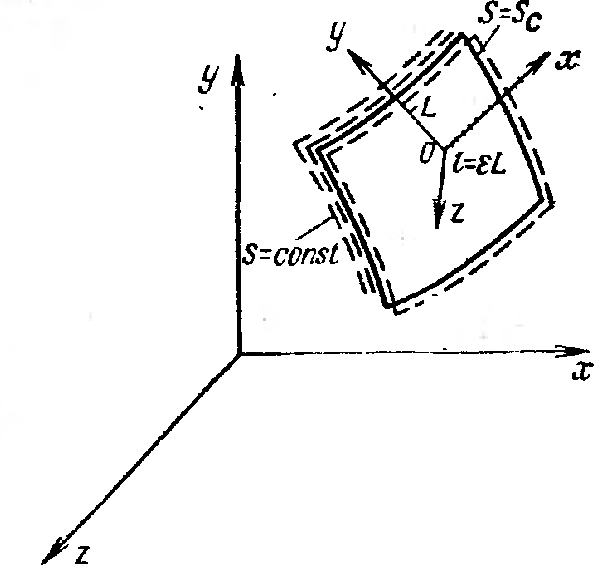
\includegraphics[width=.55\linewidth]{figures/fig-VI-10.png}\caption{}\label{q12:fig-VI-10}\end{figure}
Запишем систему уравнений в безразмерном виде. Обобщенный закон Дарси:
\begin{equation}\begin{aligned}
U_{1X}&=-\frac1\varepsilon f_1(s)\frac{\partial P_1}{\partial X},&U_{2X}&=-\frac{\mu_0}{\varepsilon}f_2(s)\frac{\partial P_2}{\partial X};\\
U_{1Y}&=-f_1(s)\frac{\partial P_1}{\partial Y},&U_{2Y}&=-\mu_0f_2(s)\frac{\partial P_2}{\partial Y};\\
U_{1Z}&=-f_1(s)\frac{\partial P_1}{\partial Z},&U_{2Z}&=-\mu_0f_2(s)\frac{\partial P_2}{\partial Z};\\
P_2-P_1&=\varepsilon J(s),&\mu_0&=\frac{\mu_1}{\mu_2}.
\end{aligned}\tag{VI.3.1}\label{q12:eq-VI-3-1}\end{equation}
Уравнения непрерывности:
\begin{equation}\begin{gathered}
m\frac{\partial s}{\partial\tau}+\frac{\partial U_{1X}}{\partial X}+\varepsilon\frac{\partial U_{1Y}}{\partial Y}+\varepsilon\frac{\partial U_{1Z}}{\partial Z}=0;\\
m\frac{\partial s}{\partial\tau}-\frac{\partial U_{2X}}{\partial X}-\varepsilon\frac{\partial U_{2Y}}{\partial Y}-\varepsilon\frac{\partial U_{2Z}}{\partial Z}=0.
\end{gathered}\tag{VI.3.2}\label{q12:eq-VI-3-2}\end{equation}
Подставляя \eqref{q12:eq-VI-3-1} в \eqref{q12:eq-VI-3-2} и отбрасывая члены порядка $\varepsilon$ и $\varepsilon^2$ получим
\begin{equation}\begin{gathered}
m\frac{\partial s}{\partial\tau}-\frac1\varepsilon\frac{\partial}{\partial X}\left(f_1(s)\frac{\partial P_1}{\partial X}\right)=0;\\
m\frac{\partial s}{\partial\tau}+\frac{\mu_0}{\varepsilon}\frac{\partial}{\partial X}\left(f_2(s)\frac{\partial P_1}{\partial X}\right)+\mu_0\frac{\partial}{\partial X}\left(f_2(s)J'(s)\frac{ds}{dX}\right)=0.
\end{gathered}\tag{VI.3.3}\label{q12:eq-VI-3-3}\end{equation}
% Источник: Barenblatt-et-al-1972.djvu; печатная страница: 166; страница файла: 168
Исключим $\partial P_1/\partial X$ из уравнений \eqref{q12:eq-VI-3-3}, что дает окончательно
\begin{equation}m\frac{\partial s}{\partial\tau}-w\frac{\partial F(s)}{\partial X}+\mu_0\frac{\partial}{\partial X}\left(f_2(s)F(s)J'(s)\frac{\partial s}{\partial X}\right)=0,\tag{VI.3.4}\label{q12:eq-VI-3-4}\end{equation}
% Знак минус перед w∂F/∂X напечатан в оригинале и сохранён.
где
\begin{equation}\begin{aligned}
w(\tau)&=\frac{u_1+u_2}{u_0}=-\frac1\varepsilon[f_1(s)+\mu_0f_2(s)]\frac{\partial P_1}{\partial X}+\mu_0f_2J'\frac{\partial s}{\partial X}=\\
&=U_{1X}+U_{2X}.
\end{aligned}\tag{VI.3.5}\label{q12:eq-VI-3-5}\end{equation}
Система \eqref{q12:eq-VI-3-1}--\eqref{q12:eq-VI-3-2} свелась к одномерному уравнению \eqref{q12:eq-VI-3-4}, потому что радиус кривизны поверхности разрыва имеет порядок $L$, и в принятом масштабе $l$ эта поверхность, как и поверхности $s=\mathrm{const}$, заменяется плоскостями. Равенство \eqref{q12:eq-VI-3-5} означает, что в пределах зоны скачка, где движение можно считать одномерным, суммарная скорость фильтрации обеих фаз вдоль оси $x$, $w$ есть величина, зависящая только от времени, как при движении в цилиндрической трубке тока.

Значение $w$ в уравнении \eqref{q12:eq-VI-3-4} находится из внешнего разложения, как безразмерная суммарная скорость фильтрации через поверхность разрыва в точке $O$. Уравнение \eqref{q12:eq-VI-3-4}, описывающее одномерное вытеснение несмешивающихся жидкостей, называется уравнением Рапопорта --- Лиса [152].

Поскольку масштаб времени во внутреннем разложении $t_1$ намного меньше, чем во внешнем, а скорость $w$ определяется внешним разложением, то при исследовании внутреннего разложения можно считать $w(\tau)=\mathrm{const}$. Ввиду различия масштабов времени во внешнем и внутреннем разложении достаточно воспользоваться стационарным решением задачи Коши для уравнения \eqref{q12:eq-VI-3-4}, т. е. положить
\begin{equation}s=s(\bar x),\quad\bar x=X-V^0\tau\quad\left(V^0=\frac{V}{u_0}\right).\tag{VI.3.6}\label{q12:eq-VI-3-6}\end{equation}
Иными словами, в масштабе времени внутреннего разложения процесс вытеснения продолжался весьма долго, и его можно считать установившимся в системе координат, связанной со скачком. При этом в силу различия масштабов $l$ и $L$ должны выполняться граничные условия
\begin{equation}s(-\infty)=s^{(1)}=s_c;\quad s(+\infty)=s^{(2)}=s_0,\tag{VI.3.7}\label{q12:eq-VI-3-7}\end{equation}
где $s^{(1)}=s_c$ и $s^{(2)}=s_0$ --- насыщенности за и перед скачком, определяемые из внешнего разложения [в задаче Баклея --- Леверетта они связаны соотношением (VI.2.30)]. Параметр $V^0$ в равенстве \eqref{q12:eq-VI-3-6} есть, очевидно, скорость распространения поверхности разрыва, определяемая формулами (VI.2.21) или (VI.2.24).

Используя \eqref{q12:eq-VI-3-6}, получим вместо \eqref{q12:eq-VI-3-4} уравнение
\begin{equation}-mV^0\frac{ds}{d\bar x}-w\frac{dF(s)}{d\bar x}+\mu_0\frac{d}{d\bar x}\left[f_2(s)F(s)J'(s)\frac{ds}{d\bar x}\right]=0.\tag{VI.3.8}\label{q12:eq-VI-3-8}\end{equation}
% Источник: Barenblatt-et-al-1972.djvu; печатная страница: 167; страница файла: 169
Интегрирование дает
\begin{equation}-mV^0s-wF(s)+\mu_0f_2(s)F_sJ'(s)\frac{ds}{d\bar x}=c=\mathrm{const}.\tag{VI.3.9}\label{q12:eq-VI-3-9}\end{equation}
% В оригинале (VI.3.9) напечатано F_s вместо F(s); сохранено.
Из условия $s=s_c$ при $\bar x\to-\infty$, учитывая, что при этом $ds/d\bar x=0$, имеем
\begin{equation}c=-mV^0s_c-wF(s_c).\tag{VI.3.10}\label{q12:eq-VI-3-10}\end{equation}
Заметим, что, поскольку значение $V$ определяется формулой (VI.2.24), второе условие \eqref{q12:eq-VI-3-7} будет выполнено автоматически. Подставляя значение $c$ из \eqref{q12:eq-VI-3-10} в \eqref{q12:eq-VI-3-9} и разрешая относительно $d\bar x/ds$, получим
\begin{equation}\frac{d\bar x}{ds}=\frac{w\mu_0f_2(s)F(s)J'(s)}{V^0(s-s_0)-[F(s)-F(s_0)]w}.\tag{VI.3.11}\label{q12:eq-VI-3-11}\end{equation}
% В числителе (VI.3.11) напечатан w, а в знаменателе отсутствует m; сохранено.
Если проинтегрировать уравнение \eqref{q12:eq-VI-3-11} по $s$, принимая начало отсчета так, чтобы при $\bar x=\bar x_1$ было $s=s_1$, где $s_0<s_1<s_c$, получим, используя для $V^0$ формулы (VI.2.24) и \eqref{q12:eq-VI-3-5} при $s^{(1)}=s_c$, $s^{(2)}=s_0$:
\[\left(V=\frac{u_0w}{m}\frac{F(s_c)-F(s_0)}{s_c-s_0};\quad V^0=\frac{w}{m}\frac{F(s_c)-F(s_0)}{s_c-s_0}\right);\]
\begin{equation}\bar x-\bar x_1=\int_{s_1}^s\frac{f_2(s)F(s)J'(s)\,ds}{[F(s_c)-F(s_0)]\dfrac{s-s_0}{s_c-s_0}-F(s)+F(s_0)}.\tag{VI.3.12}\label{q12:eq-VI-3-12}\end{equation}
Если справедливо предположение о стационарности скачка насыщенности и $V$ определяется из формулы (VI.2.24), получим иную запись для $\bar x(s)$:
\begin{equation}\bar x-\bar x_1=\int_{s_1}^s\frac{f_2(s)F(s)J'(s)\,ds}{F'(s_c)(s-s_0)-F(s)+F(s_0)}.\tag{VI.3.13}\label{q12:eq-VI-3-13}\end{equation}
Интегралы \eqref{q12:eq-VI-3-12} и \eqref{q12:eq-VI-3-13} описывают переходную зону бесконечной протяженности, что является следствием принятой аппроксимации. Фактически для определения ширины зоны нужно брать по формулам \eqref{q12:eq-VI-3-12} и \eqref{q12:eq-VI-3-13} расстояние между точками с насыщенностями $s_0+\delta$ и $s_0-\delta$, где $\delta$ --- малая, но конечная величина. Тогда безразмерная ширина переходной зоны будет порядка нескольких единиц, а размерная ширина --- порядка $l$, т. е. $\dfrac{p_c^0}{\Delta p}L$ или $\dfrac{\alpha\sqrt{k}}{\mu_1u_0}$. Типичная кривая распределения насыщенности в переходной зоне приведена на рис. \ref{q12:fig-VI-11}.
% В оригинале здесь s_0+δ и s_0−δ; не исправлено на s_c−δ.

% Источник: Barenblatt-et-al-1972.djvu; печатная страница: 168; страница файла: 170
\begin{figure}[H]\centering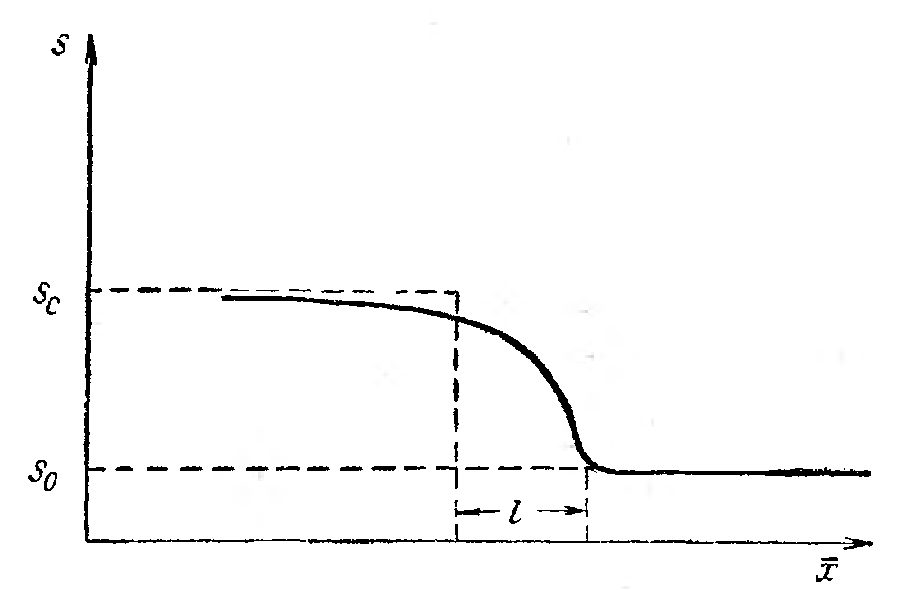
\includegraphics[width=.75\linewidth]{figures/fig-VI-11.png}\caption{}\label{q12:fig-VI-11}\end{figure}

\end{document}
